\chapter{Terminologies}

\begin{itemize}
	\item Le client est le commanditaire du projet.
	\item Un utilisateur est une personne souhaitant utiliser un logiciel du client. 
	\item Une licence est un droit accordé pour une machine et un utilisateur d'utiliser un logiciel donné.
\end{itemize}

\chapter{Contexte du projet}

Ce projet s’intitulant “Gestion et protection de licence” est proposé par notre client \\M.
Ziadi.\newline

Il a pour but de créer une ou plusieurs applications de gestion, génération et protection 
de licence, plus particulièrement un gestionnaire de licence pour les logiciels créés par monsieur
Ziadi.\newline

Dans notre cas ce projet a pour but de nous apporter des connaissances et de l'expérience dans les domaines traités  mais aussi de valider notre $1^{ere}$ année de Master Informatique en Sécurité des Systèmes d’Information (SSI).\newline

Nous pouvons être amenés à travailler avec M. Macadré pour tout ce qui est
serveur et gestion de machine virtuelle (pour leurs mise en place).

Nous nous appuyons sur la Spécification Technique de Besoin, le Document d'Architecture
Logicielle, le Cahier de Recette, l’Analyse des Risques, et sur ce Plan de Développement
pour conduire le projet.

\chapter{Méthodologie de développement}

Depuis le début du projet nous travaillons selon un fonctionnement agile, avec des
réunions et des livrables réguliers, avec le client. Ce fonctionnement permet de produire de
la valeur rapidement.\newline

Nous avons choisi de commencer le développement de l’application par les vues car
nous sommes partis du principe que le but final de ce projet était de rendre une application,
avec des rendus tout au long du semestre. Commencer par les vues nous permettra d’avoir
un visuel le plus rapidement possible, et d’obtenir un prototype manipulable, pour l’ensemble
des livrables.\newline

Ces prototypes ne contiendront bien sûr pas l’ensemble des fonctionnalités finales
attendues par le client, mais nous permettront de réagir plus rapidement sur l’ajout de
fonctionnalités dans l’application, en fonction des demandes de ce dernier, mais nous
permettra également de faire les tests plus simplement en nous assurant que
les vues sont correctement implémentées.\newline

Après avoir implémenté les vues qui permettent de naviguer entre elles, nous
commencerons par implémenter le modèle de protection et de gestion des licences.\newline

La sécurité étant au coeur de notre projet, les éléments tel que l'obfuscation, l'injection de code
et la partie gestion et sécurisation de base de données seront des éléments pouvant être gérés en
divisant nos ressources car ils sont facilement intégrable au projet final.

\chapter{Organisation et responsabilités}

Pour organiser ce projet et travailler efficacement, nous avons affecté un rôle à
chacun. Néanmoins, tous les acteurs de ce projet auront les rôles de développeur et de
rédacteur. Voici notre organigramme :\newline

\begin{figure}[!h]
    \centering
    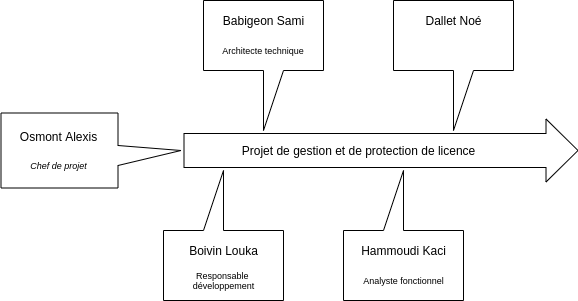
\includegraphics[width=15cm]{schema_role_projet.png}
\end{figure}

\begin{itemize}
	\item  \textbf{Chef de projet :} \newline
	\begin{itemize}
		\item Organiser et conduire le projet de bout en bout.
		\item Décide des actions et résout les désaccords entre les membres du projet.\newline
	\end{itemize}

	\item \textbf{Architecte tehcnique :} \newline
	\begin{itemize}
		\item Garantit l'encadrement et la maintenance technique du projet.
		\item Assure la fiabilité, la performance et l'évolution du système d'information.\newline
	\end{itemize}
	\newpage

	\item \textbf{Analyste fonctionnel :} \newline
	\begin{itemize}
		\item Schématise l’interface de l’application.
		\item Se charge de la conception générale de l’interface, de la clarté de la
		navigation, de l’optimisation des parcours ainsi que de la qualité des
		contenus.\newline
	\end{itemize}
	
	\item \textbf{Responsable développement :} \newline
	\begin{itemize}
		\item Définit les besoins du client.
		\item Assure le suivi fonctionnel.\newline
	\end{itemize}
\end{itemize}

\chapter{Organigramme des tâches}
L'organigramme des tâches présent ci-dessous n'est qu'une capture du momment. En effet celui-ci sera mis à jour en fonction 
des possibles nouvelles tâches qui viendront le compléter.\newline

L'organigramme est disponible en annexe pour une meilleur lisibilité.\newline

\begin{figure}[!h]
    \centering
    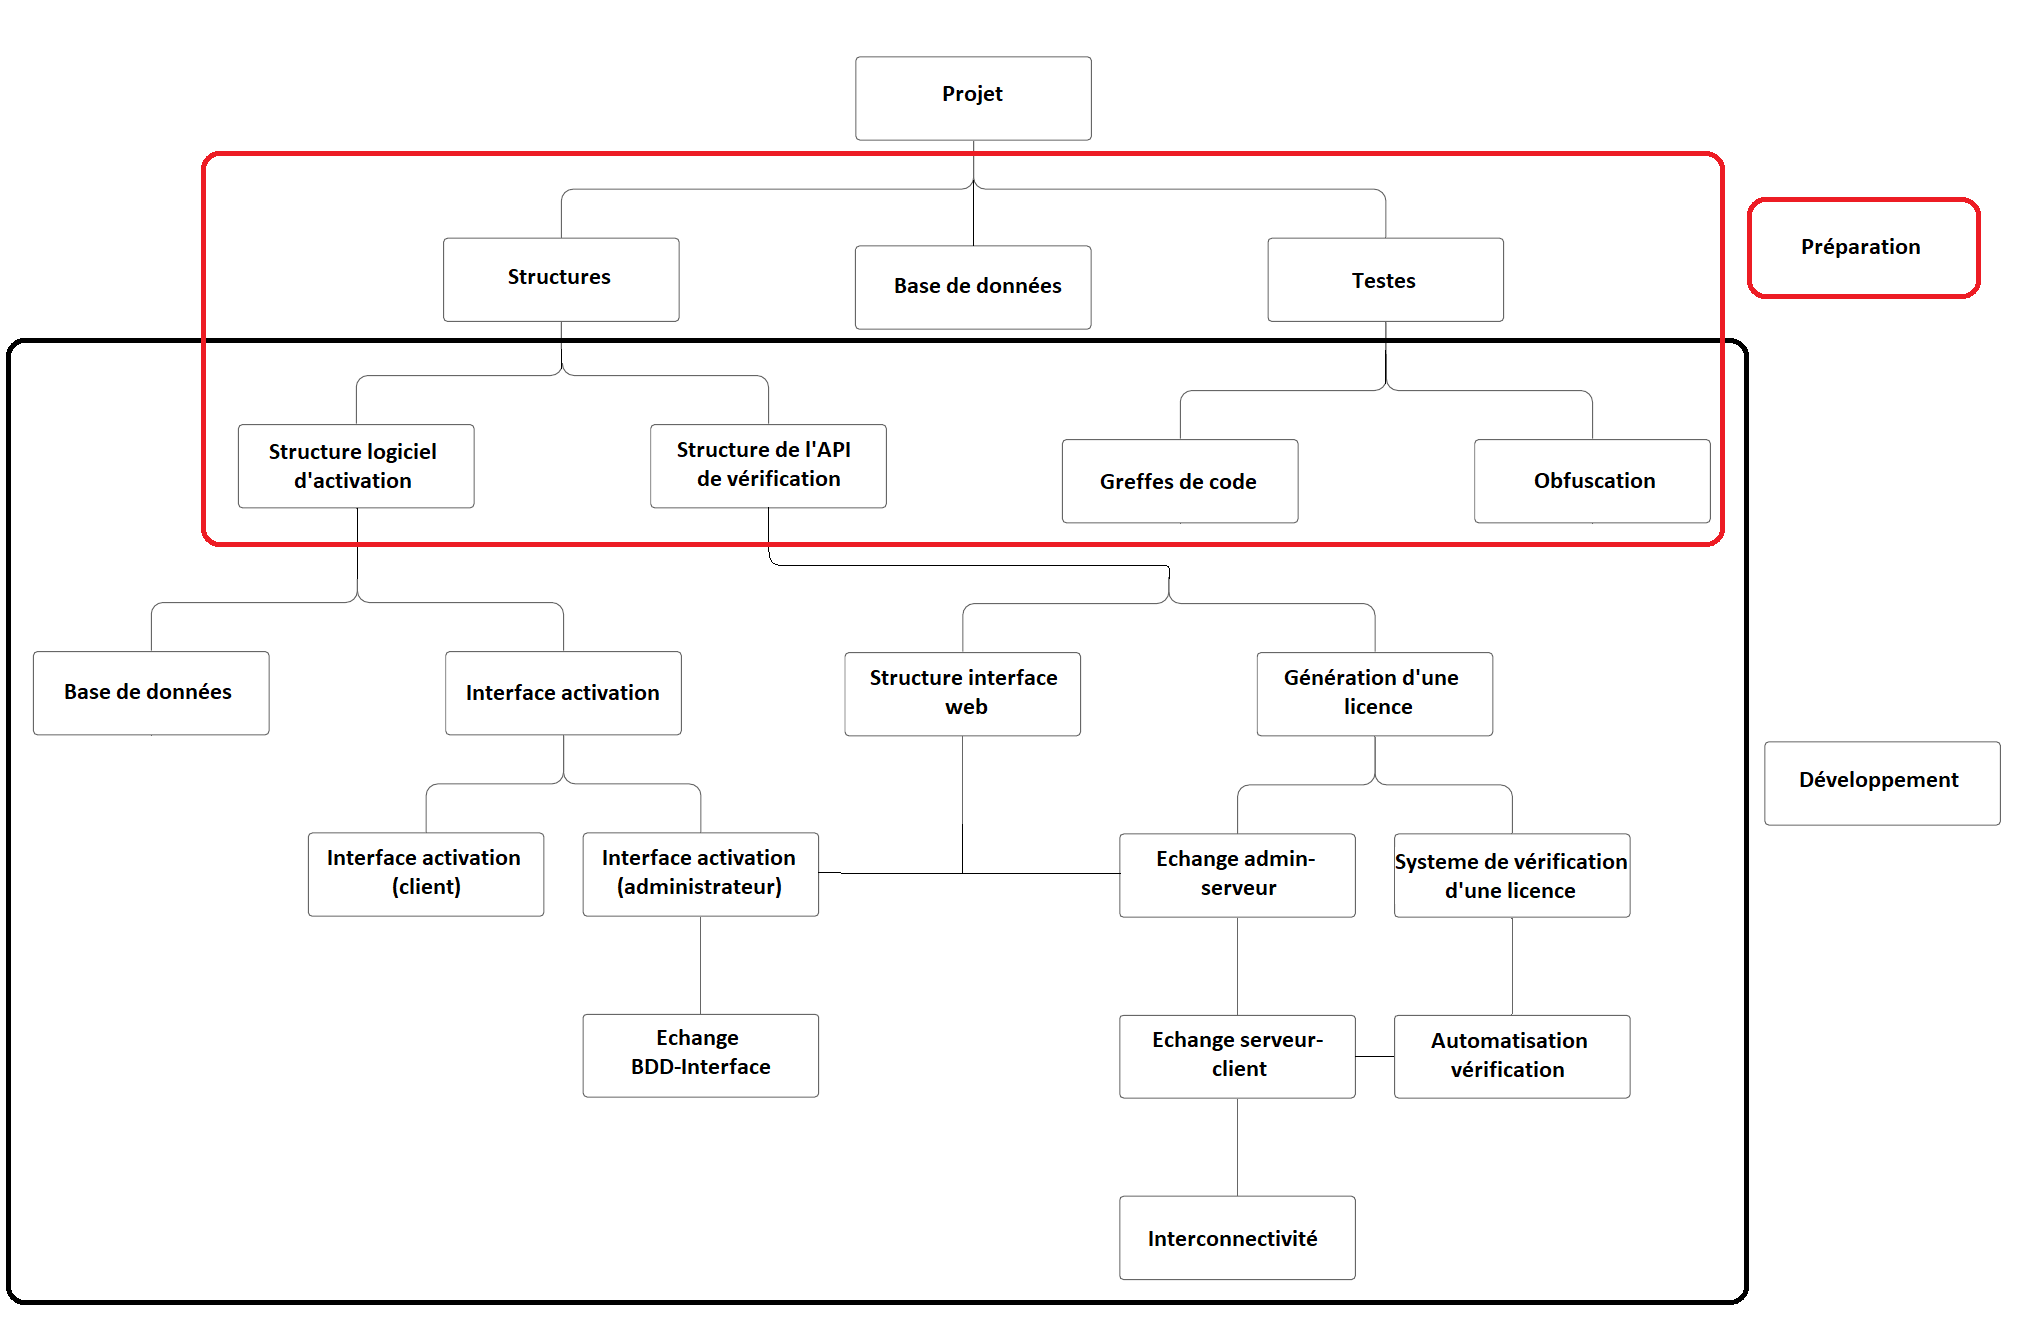
\includegraphics[width=18cm]{organi.png}
\end{figure}

\chapter{Évaluation du projet et dimensionnement des moyens}

\section{Charge et répartition par phase}
Nous avons divisé la charge et la répartition par phase. La première phase est intitulée
«Préparation». Cette première phase permet de donner un temps aproximatif de structuration du
projet, de vérification des répartitions des tâches et des phases de tests qui permettront des
évaluations de temps de développement plus précises tel que les tests de greffe de code ou ceux
d'obfuscation. Cette phase, d'après nos estimations, nécessiterait 4 semaines, 2 semaines de
répartition et de tests puis 2 semaines de structure de projet qui se terminerait par une
réunion avec le client pour attester de l'evaluation du temps
et des ressources nécessaires au bon déroulement du projet.\newline
\newline

La seconde phase est celle du développement qui nécessitera le plus de temps. En effet nous avons évalué cette phase à deux mois de travail.
Cette phase se decomposerait en 3 parties : \newline

\begin{itemize}
	\item Phase post-préparation : 2 semaines\\ 
	    Cette phase est nécessaire pour structurer le projet et les parties de développement avant
        la séparation des tâches principale, En effet après la phase de préparation il nous faut
        créer une structure de projet pour que chaque personne puisse travailler sur des bases
        solides sans géner l'avancement sur les parties des autres membres du projet. \newline
	\item Phase de développement : 4 semaines\\
	    La phase de développement est quant à elle la principale, elle consiste à repondre aux
        besoins de chaque élément du projet. Cette phase permet à tous les différents éléments
        d'être fonctionnel.
	\item Phase d'interaction : 3 semaines\\
	    La derniere phase consiste à connecter tous ces développements, le coeur de cette partie
        sera donc de connecter les éléments entre eux. (serveur $\rightarrow$ administrateur;
        téléchargement du logiciel d'activation $\rightarrow$ client; ...)
\end{itemize}
\newpage

\section{Besoin en moyens et en ressources}
Nécessaire au développement et tests:
\begin{itemize}
	\item Serveur
	\item Base de données
	\item Logiciels du client
	\item Dépot(s) Git\newline
\end{itemize}
\medskip

Après une concertation entre les membres du projet et leurs connaissances personnelles,
l'estimation de temps fait est de 110 heures en moyenne de travail afin de remplir les exigences
du client, nos exigences personnelles et de terminer les tâches définis	dans l'organigramme
ci-dessus.\newline
\medskip

Remarque : Le chapitre ci-dessus «Évaluation du projet et dimensionnement des moyens» est à titre
indicatif, en effet ce chapitre comme le chapitre précédent n'est qu'une évaluation. Ils seront
donc amenés à changer au cours du développement du projet.

\chapter{Planning général}

\section{Diagramme de Gantt}

Le diagramme de Gantt présent ci-dessous n'est qu'une capture du moment. En effet celui-ci sera
mis à jour en fonction de l'avancement du projet, de la répartition des tâches et des possibles
nouvelles tâches qui viendront le compléter.\newline

Le diagramme de Gantt est disponible en annexe.

\begin{figure}[!h]
    \centering
    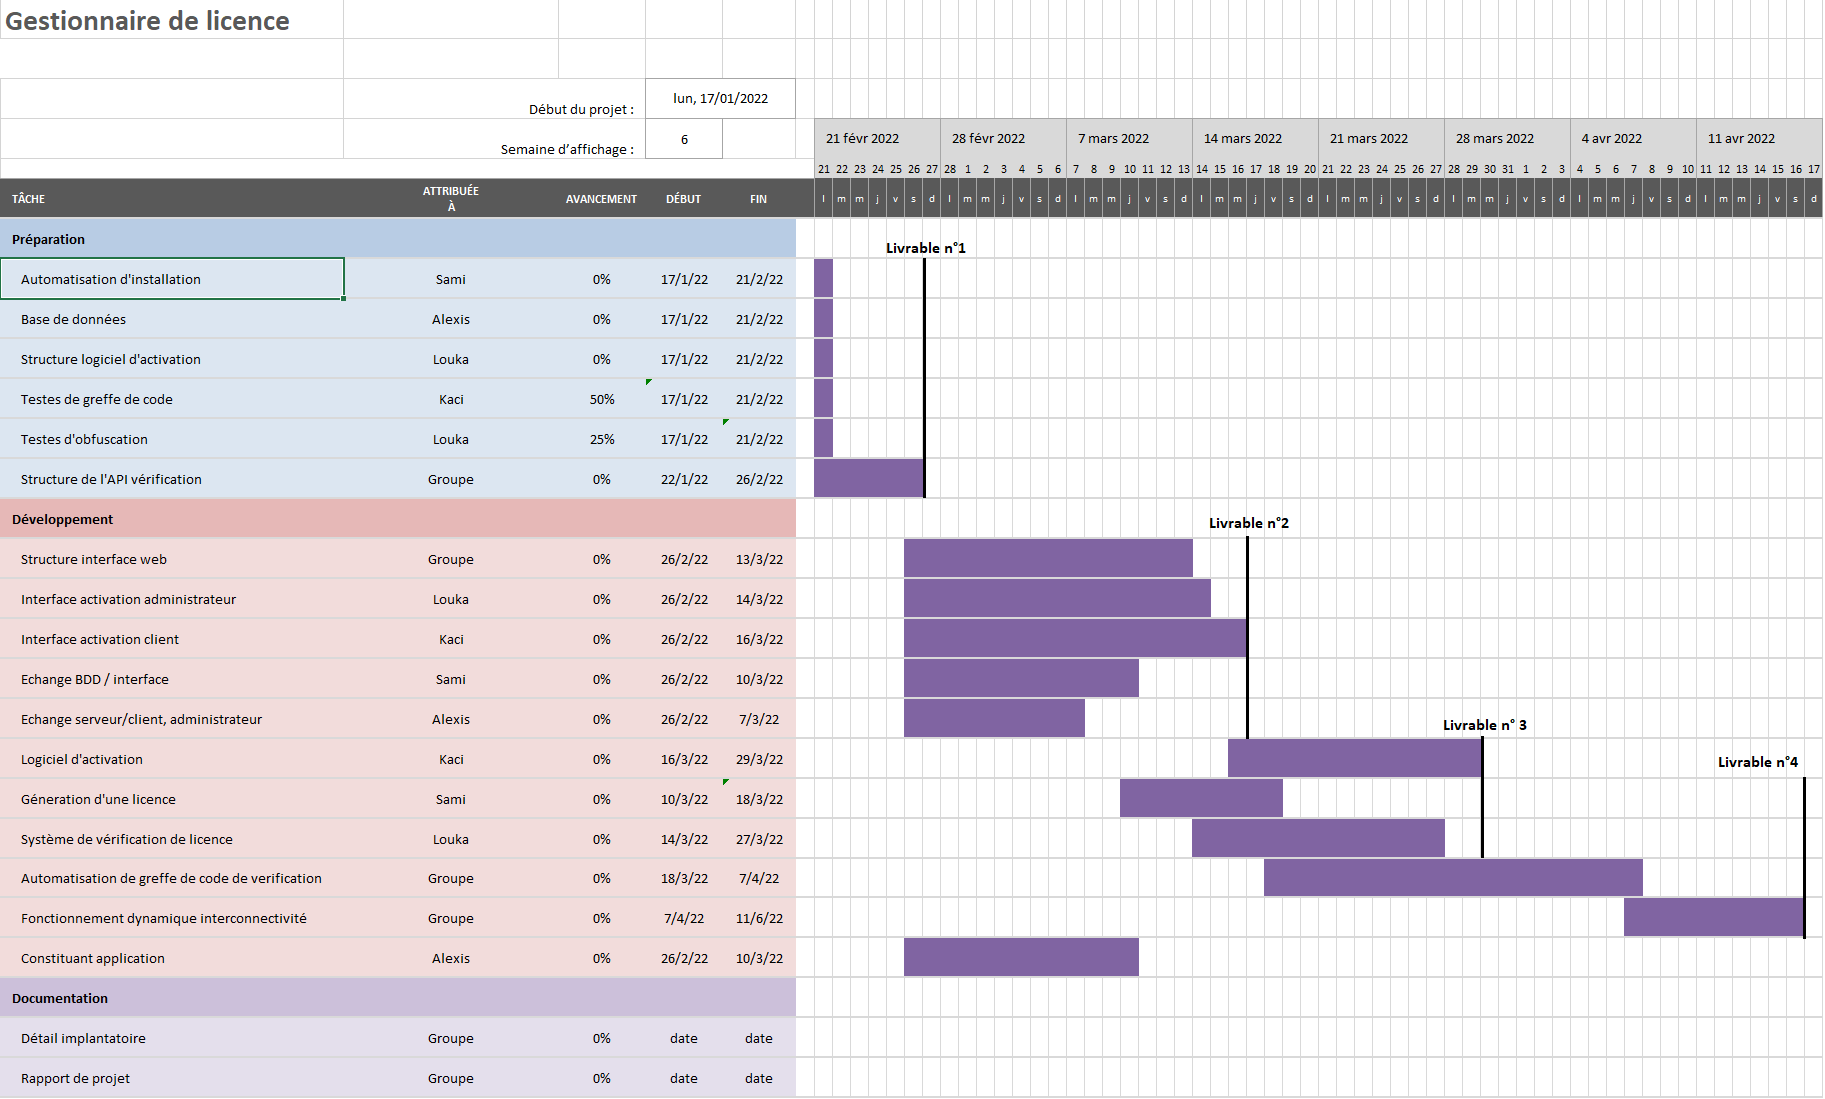
\includegraphics[width=17cm]{Gantt.png}
\end{figure}

\section{Livrables}
\begin{itemize}
	\item Livrable n°1 : Démonstration
	\item Livrable n°2 : Activation de licence
	\item Livrable n°3 : Génération et vérification de licence
	\item Livrable n°4 : Projet abouti
\end{itemize}

\chapter{Procédés de gestion}

\section{Gestion de la documentation}
Au second semestre, nous devrons fournir les documents suivants :

\begin{itemize}
    \item Documentation technique : décrit le fonctionnement détaillé de l’application.
    \item Notice d’utilisation : support explicatif du maniement de l’application.
    \item Des comptes rendus post-réunion après chaque réunion.
    \item Des livrables pré-réunion chaque deux semaines.\\ \newline
\end{itemize}

\section{Gestion des configurations}
Lors du développement, nous utiliserons le GitLab fourni par l’université ainsi que GitHub. Chacun
aura une tache de développement et il y aura des réunions de travail en groupe qui donneront les
versions stables du code (pré-réunion) et des documentations (en \LaTeX). Chacun aura son espace
pour permettre à tous de fusionner sa partie à la branche principale.


\chapter{Revues et points clefs}

L'objectif dans notre cas est de faire suivre notre projet par notre client,
nous fournirons donc au client un livrable toutes les deux semaines, et nous effectuerons
quelques jours après chaque livraison une réunion avec lui pour voir les modifications à
apportées. Des dates prévisionnelles ont été indiquées dans le diagramme de Gantt.\newline

Comme précisé dans la partie «Évaluation du projet et dimensionnement des moyens» une réunion sera
organisée à chaque fin de phase pour faire une revues des points clefs du projet et pour informer
le client de l'avancement du projet et de ses besoins.

\chapter{Procédure de suivi d'avancement}

Pour avancer rapidement et efficacement tout en évitant les hors-sujets, nous avons
décidé d’utiliser diverses plateformes pour suivre l’avancement de chacun, et de ce fait,
d’éviter qu’un membre ne soit en attente. Les plateformes utilisées sont les suivantes :\newline

\begin{itemize}
	\item Discord :\\
	Cet outil nous permet de communiquer rapidement entre nous et
    de faire des audios / visioconférences pour nos réunions. Il est aussi très utile
    pour communiquer rapidement et faire des annonces importantes (réunions,
    vérification d’un mail avant son envoi, etc.) et pour partager / archiver les
    comptes rendus de toutes les réunions.\\
	
    \item Trello :\\
	Cet outil nous permet de répartir et de savoir sur quelle tâche
    travaillent les membres de l’équipe et de connaître leur avancement.\\
	
    \item GitHub :\\
	L’université nous a fourni cet outil qui est très pratique pour stocker
    les documentations produites et le code source de l’application que nous
    aurons à faire lors de la phase de développement.\\
	
    \item Google docs / GitHub :\\
	Ces outils nous permettent de réaliser les documents demandés
    pour la matière Gestion de Projet. Google Docs nous permet de travailler à
    plusieurs sur un même document. Les modifications apparaissent en temps
    réel et sont sauvegardées sur une période de trente jours. Il est donc possible
    de consulter des versions antérieures de nos documents en quelques clics.\\
	
    \item Réunions :\\
	Le meilleur moyen de travailler efficacement reste le fait d'organiser des réunions en physique 
	plutôt que des appels ou des échanges de messages. C'est pourquoi nous organisons régulièrement
    des réunions entre membre du projet pour faire un point, définir les objectifs et avancer sur
    le projet. \newline
\end{itemize}

Pour tenir de l'avancement du projet nous planifions des séances de travails et des réunions
hebdomadaires pour traiter aussi bien de l'aspect technique que de l'aspect gestion de projet.
Des comptes rendu de réunion sont effectués après chaqu'une d'entre elles.
